\documentclass[a4paper,12pt,oneside]{article}
\usepackage{graphicx}
\usepackage{hyperref}
\usepackage[T1]{fontenc}
\usepackage[utf8]{inputenc}
\usepackage{setspace}
\usepackage{amsmath}
\usepackage{amssymb}

\begin{document}

    \thispagestyle{plain}
    \begin{center}
        \normalsize
        \textbf{Assignment 1}
            
        \vspace{0.2cm}
        \normalsize
        21/10/2022
            
        \vspace{0.2cm}
        \textbf{Francesco Refolli 865955}
    \end{center}

    \section{Esercizio 1}

    \begin{align}
        \text{$max \; x_1 + x_2$} \\
        \text{$x_1 + x_2 \leq 2$} \\
        \text{$2 x_1 - x_2 \leq 0$} \\
        \text{$x_1, x_2 \geq 0$}
    \end{align}

    Costruisco il grafico con le equazioni dei vincoli lungo l'asse $x_1 \times x_2$.
    Riscrivo per comodita' i primi due vincoli in forma equivalente:

    \begin{align}
        \text{$x_1 \leq 2 - x_2$} \\
        \text{$x_1 \leq \frac {x_2} 2$}
    \end{align}

    \begin{center}
        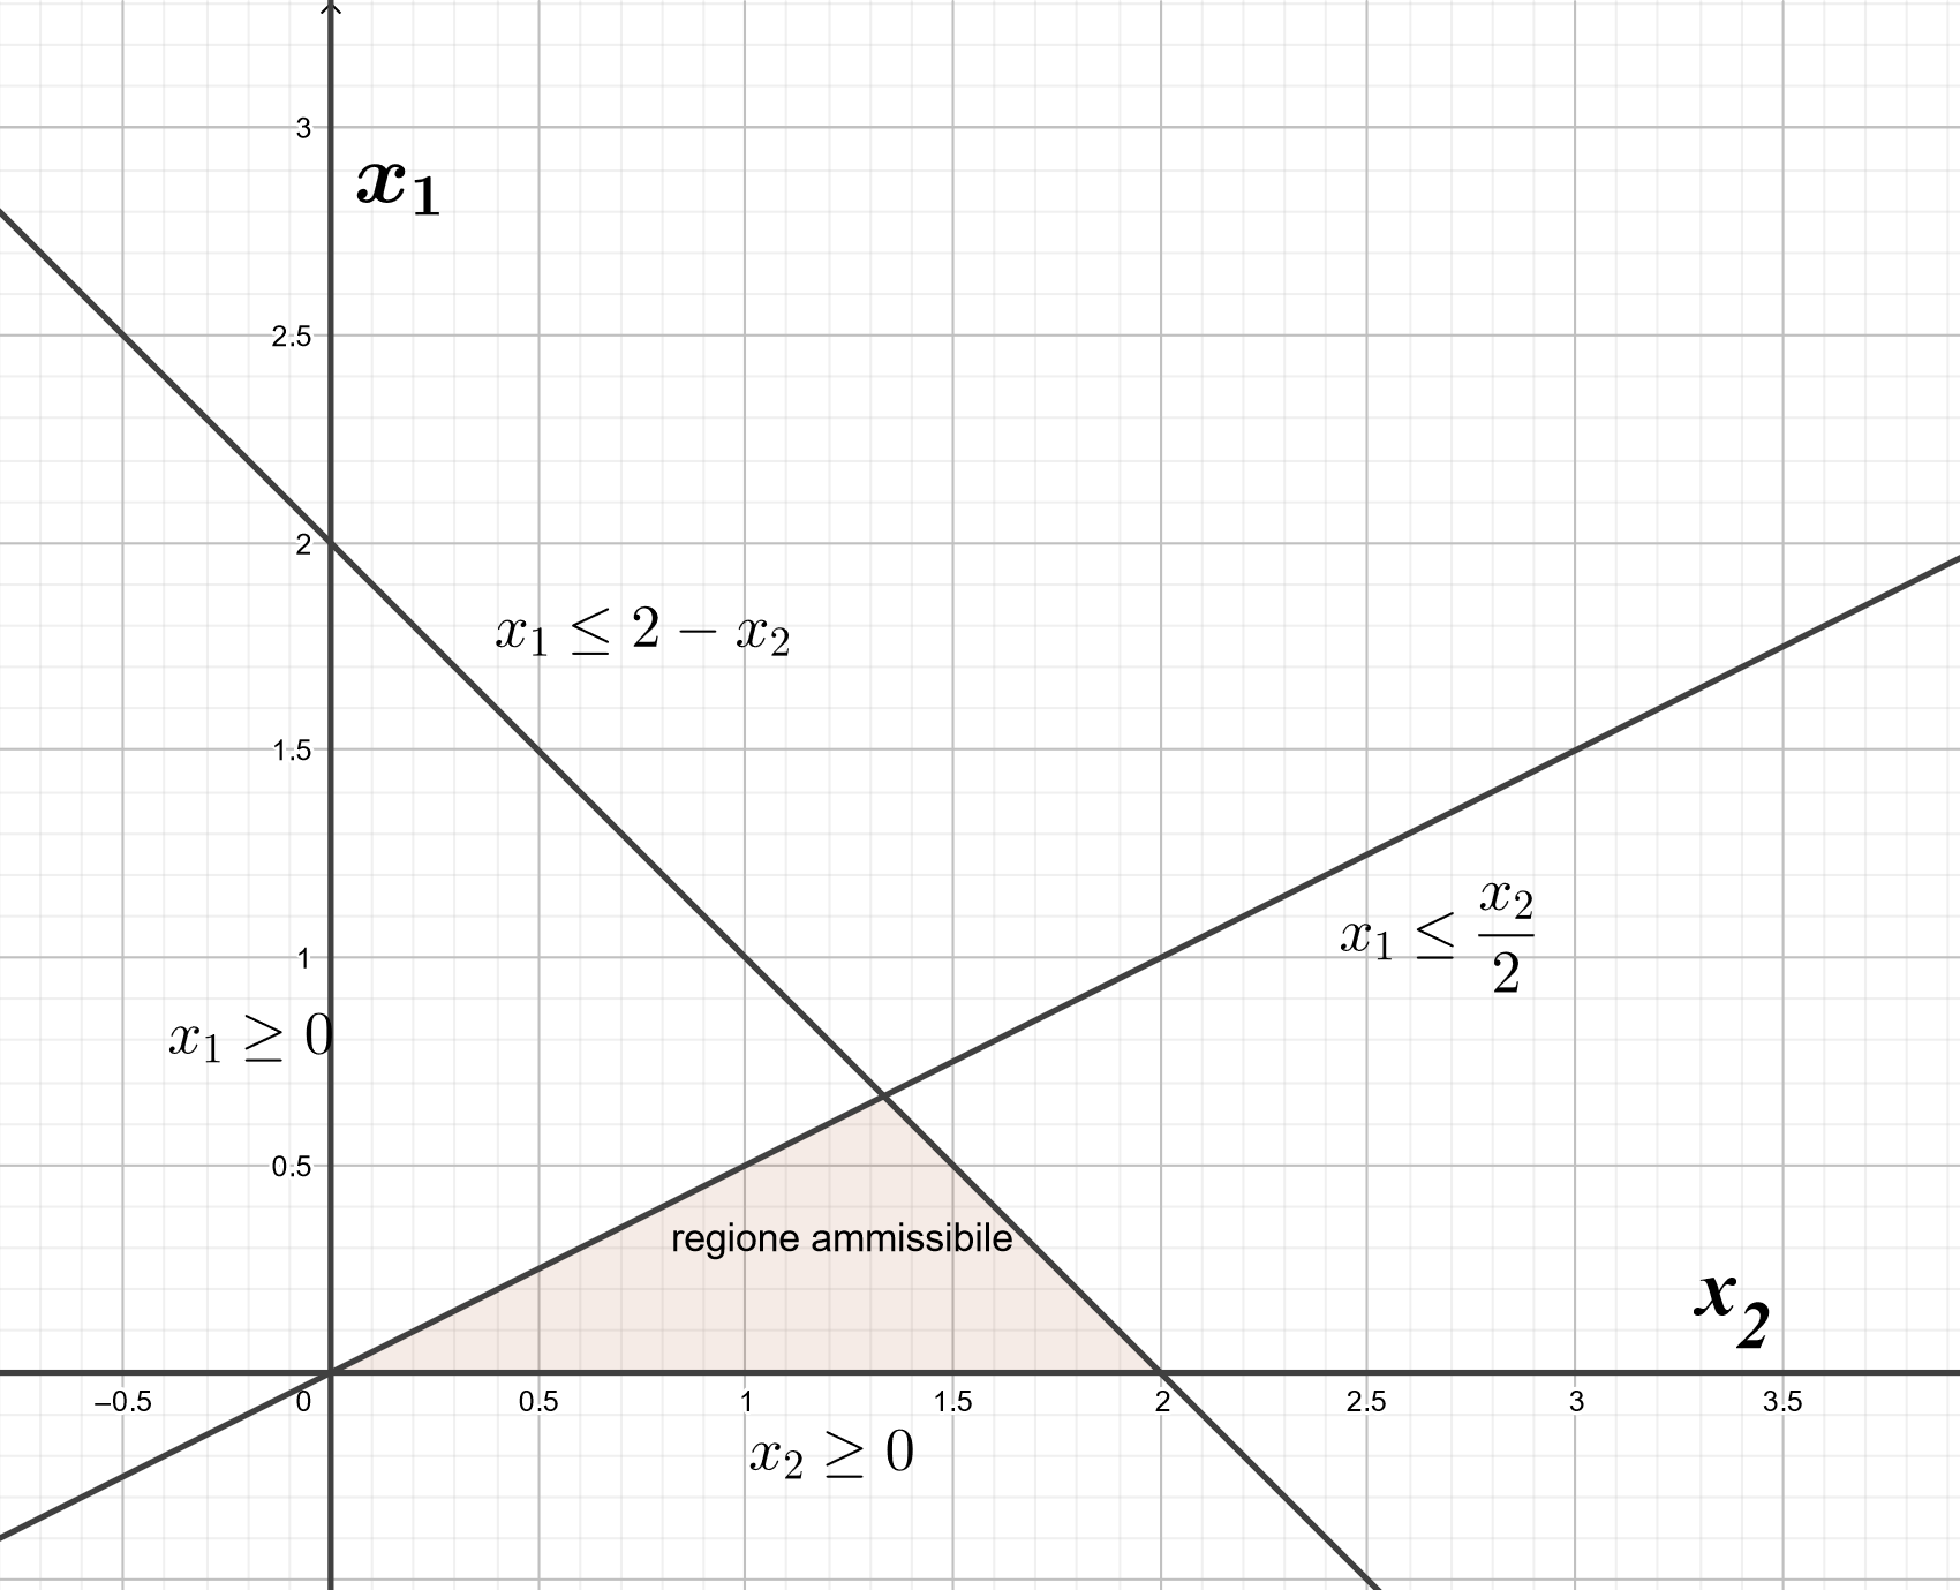
\includegraphics[width=12cm]{prima-fase.png}
    \end{center}

    Quindi disegno il gradiente della funzione obiettivo $g$ e la funzione obiettivo.

    \begin{center}
        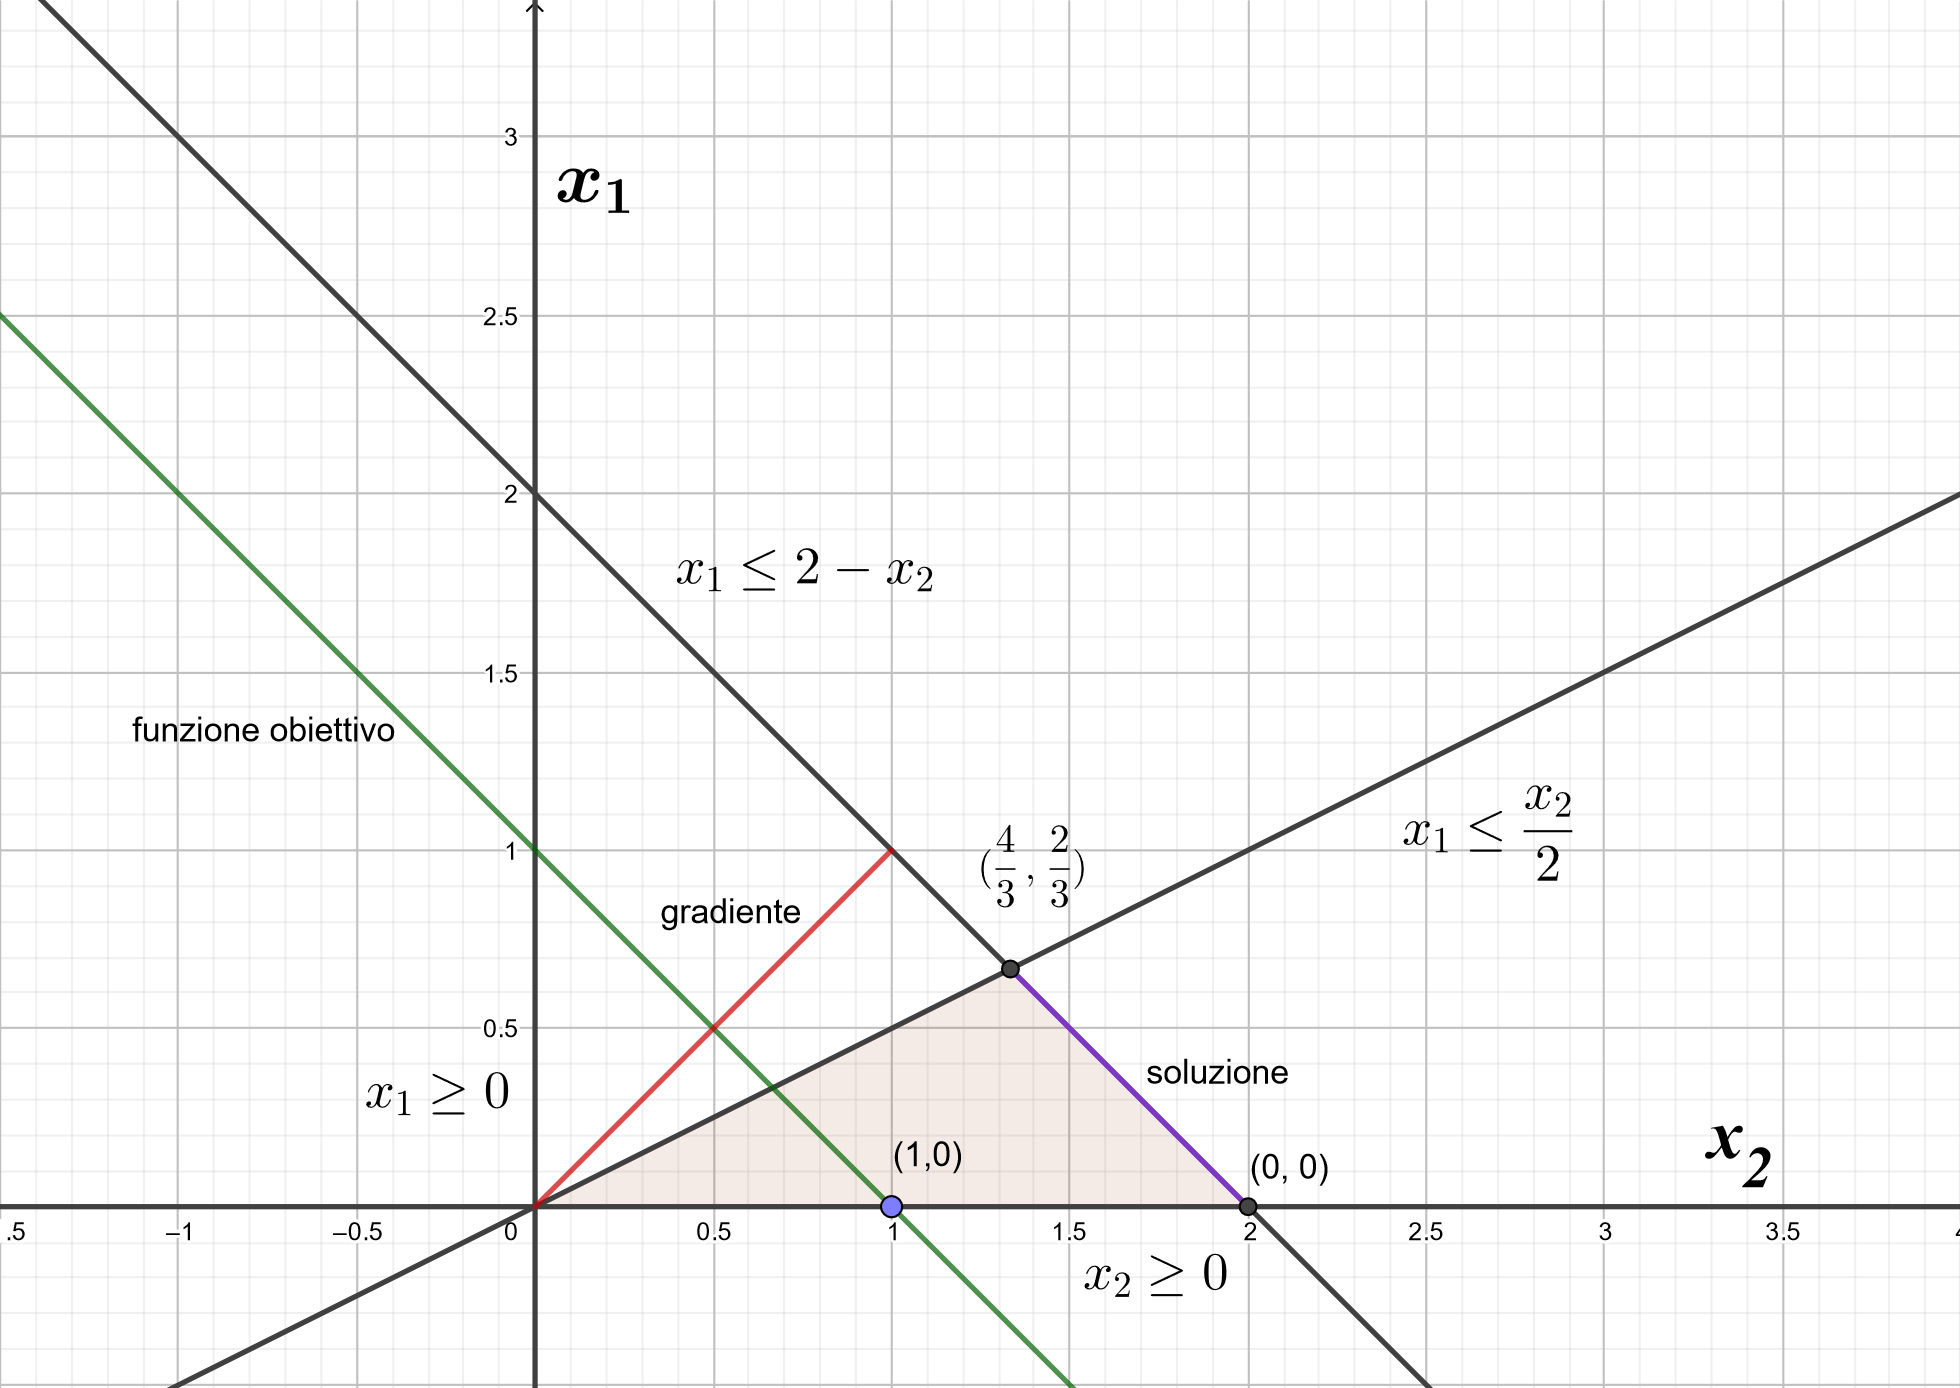
\includegraphics[width=12cm]{seconda-fase.png}
    \end{center}

    Il vettore del gradiente della funzione obiettivo $g$ = <$1, 1$> , composto dalle derivate parziali delle componenti della funzione obiettivo, e' perpedincolare al vincolo $x_1 \leq 2 - x_2$.
    Il problema ha \textbf{Infinite Soluzioni Ottime}.
    Le soluzioni sono tutte le coppie <$x_1, x_2$> che risiedono nello spigolo della regione obiettivo su cui si poggia il vincolo $x_1 \leq 2 - x_2$.
    Per calcolare il segmento e' sufficiente calcolare l'intersezione dei vincoli $x_1 \leq 2 - x_2$ e $x_2 \geq 0$.
    Il risultato sono i punti: ($0, 2$),  ($\frac 2 3, \frac 4 3$). Le soluzioni sono tutti i punti compresi nel segmento delimitato da essi.

    \newpage

    \section{Esercizio 2}

    \begin{align}
        \text{$max \; x_1 + x_2$} \\
        \text{$x_1 + x_2 - x_3 = 2$} \\
        \text{$2 x_1 - x_2 \leq 0$} \\
        \text{$x_1, x_2 \geq 0$} \\
        \text{$x_3 \leq 0$}
    \end{align}

    \paragraph{Conversione in forma aumentata}

    \subparagraph{1}

    La forma aumentata non prevede vincoli di non positivita', quindi inverto il segno di $x_3$ in tutti i vincoli:

    \begin{align}
        \text{$max \; x_1 + x_2$} \\
        \text{$x_1 + x_2 + x_3 = 2$} \\
        \text{$2 x_1 - x_2 \leq 0$} \\
        \text{$x_1, x_2, x_3 \geq 0$}
    \end{align}

    \subparagraph{2}

    Aggiungo una variabile di slack $x_4$ per portare il vincolo $\leq$ in vincolo $=$.

    \begin{align}
        \text{$max \; x_1 + x_2$} \\
        \text{$x_1 + x_2 + x_3 = 2$} \\
        \text{$2 x_1 - x_2 + x_4 = 0$} \\
        \text{$x_1, x_2, x_3, x_4 \geq 0$}
    \end{align}

    \subparagraph{3}

    Quindi esporto la funzione obiettivo $f(x)$ in un vincolo $Z - f(x) = 0$.

    \begin{align}
        \text{$max \; Z$} \\
        \text{$Z - x_1 - x_2 = 0$} \\
        \text{$x_1 + x_2 + x_3 = 2$} \\
        \text{$2 x_1 - x_2 + x_4 = 0$} \\
        \text{$x_1, x_2, x_3, x_4 \geq 0$}
     \end{align}

    \paragraph{Risoluzione con tableau}

    Riempio la forma tabellare con i coefficienti delle variabili nei vincoli e nella funzione obiettivo.
    La tabella risulta: \\

    \begin{center}
        \begin{tabular}{|c|c|c|c|c|c|c|}
            \hline
            base & Z & $x_1$ & $x_2$ & $x_3$ & $x_4$ & b\\
            \hline
            Z & 1 & -1 & -1 & 0 & 0 & 0\\
            3 & 0 & 1 & 1 & 1 & 0 & 2\\
            4 & 0 & 2 & -1 & 0 & 1 & 0\\
            \hline
        \end{tabular}
    \end{center}

    La base e' formata da 2 variabili, perche' il numero di vincoli e' proprio 2.
    Inserisco nella base le variabili $x_3$, $x_4$. Fuori base rimangono $x_1$, $x_2$.
    La soluzione di base corrente <$x_1$,$x_2$,$x_3$,$x_4$> = <0,0,2,0> e' ammissibile. Quindi procedo con l'algoritmo del simplesso.

    \paragraph{iterazione 1}

    Non esiste un coefficiente in prima riga negativo piu' basso di tutti gli altri. Scelgo la colonna 1 con coefficiente $-1$.
    La riga 2 ha il rapporto minimo, diventa la riga pivot.
    Il valore pivot e' $2$, moltiplico tutta la riga 2 per $\frac 1 2$ per ridurre il valore pivot a $1$.
    Quindi applico l'algoritmo per ricalcolare la tabella.
    Questa iterazione ha l'effetto di scambiare $x_4$ della base con $x_1$.

    \begin{center}
        \begin{tabular}{|c|c|c|c|c|c|c|}
            \hline
            base & Z & $x_1$ & $x_2$ & $x_3$ & $x_4$ & b\\
            \hline
            Z & 1 & 0 & -$\frac 3 2$ & 0 & $\frac 1 2$ & 0\\
            3 & 0 & 0 & $\frac 3 2$ & 1 & -$\frac 1 2$ & 2\\
            1 & 0 & 1 & -$\frac 1 2$ & 0 & $\frac 1 2$ & 0\\
            \hline
        \end{tabular}
    \end{center}

    \paragraph{iterazione 2}

    Scelgo la colonna 2 perche' possiede il coefficiente in prima riga negativo piu' basso, ovvero -$\frac 3 2$.
    La riga 1 ha il rapporto minimo, diventa la riga pivot.
    Il valore pivot e' $\frac 3 2$, moltiplico tutta la riga 2 per $\frac 2 3$ per ridurre il valore pivot a $1$.
    Applico l'algoritmo per ricalcolare la tabella.
    Questo ha l'effetto di scambiare $x_3$ della base con $x_2$.

    \begin{center}
        \begin{tabular}{|c|c|c|c|c|c|c|}
            \hline
            base & Z & $x_1$ & $x_2$ & $x_3$ & $x_4$ & b\\
            \hline
            Z & 1 & 0 & 0 & 1 & 0 & 2\\
            2 & 0 & 0 & 1 & $\frac 2 3$ & -$\frac 1 3$ & $\frac 4 3$\\
            1 & 0 & 1 & 0 & $\frac 1 3$ & $\frac 1 3$ & $\frac 2 3$\\
            \hline
        \end{tabular}
    \end{center}

    \paragraph{iterazione 3}

    La prima riga non contiene piu' valori negativi, l'algoritmo del simplesso si arresta. \\
    La soluzione di base corrente e' <$x_1$,$x_2$,$x_3$,$x_4$> = <$\frac 2 3$,$\frac 4 3$,0,0> \\
    Quindi una soluzione al problema PL e' <$x_1$,$x_2$> = <$\frac 2 3$,$\frac 4 3$>\*

    Ad ogni modo, siccome una delle variabili non di base ha coefficiente 0 in prima posizione e' possibile continuare con le iterazioni per individuare una ulteriore soluzione ottimale al problema PL. \\

    Selezionando la colonna $x_4$, l'unica riga con coefficiente positivo e' la riga 2. Quindi moltiplico la stessa per l'inverso del numero pivot: $(\frac 1 3)^{-1} = 3$.
    Successivamente ricalcolo le altre righe di conseguenza.

    Risulta:

    \begin{center}
        \begin{tabular}{|c|c|c|c|c|c|c|}
            \hline
            base & Z & $x_1$ & $x_2$ & $x_3$ & $x_4$ & b\\
            \hline
            Z & 1 & 0 & 0 & 1 & 0 & 2\\
            2 & 0 & 1 & 1 & 1 & 0 & 2\\
            4 & 0 & 3 & 0 & 1 & 1 & 2\\
            \hline
        \end{tabular}
    \end{center}

    \paragraph{iterazione 3}

    La prima riga non contiene piu' valori negativi, l'algoritmo del simplesso si arresta. \\
    La soluzione di base corrente e' <$x_1$,$x_2$,$x_3$,$x_4$> = <0,2,0,2> \\
    Quindi un'altra soluzione al problema PL e' <$x_1$,$x_2$> = <0,2>\*
\end{document}
